\documentclass[svgnames,12pt,aspectratio=149]{beamer}
\mode<presentation>%
{
  \usetheme{Boadilla}
  \setbeamercovered{dynamic}
}
\usepackage[english,spanish]{babel}
\usepackage[utf8]{inputenc}
\usepackage[T1]{fontenc}
\usepackage{sty/BeamerLille}
\usepackage{float}
\usepackage{caption}
\usepackage{subfigure} 
\usepackage{quantikz}
\usepackage{graphicx}
\usepackage{dsfont}
\graphicspath{ {./images/} }
\usepackage{tikz}
\renewcommand\qedsymbol{$\blacksquare$}
\newcommand{\ra}{\rangle}
\newcommand{\la}{\langle}
\newcommand{\rala}{\rangle\langle}
\newcommand{\tr}{{\rm Tr}}
\newcommand{\E}{\mathcal{E}}
\newcommand{\tensor}{\otimes}
\newcommand{\prodtensor}{\bigotimes_{i=1}^{N}}
\newcommand{\fuzzy}[1]{\mathcal{F}\left(#1\right)}
\newcommand{\fuzzydagger}[1]{\mathcal{F}^{\dagger}\left(#1\right)}
\newcommand{\permut}[2]{\Pi_{#1}#2\Pi_{#1}^{\dagger}}
\newcommand{\permutdagger}[2]{\Pi_{#1}^{\dagger}#2\Pi_{#1}}


\usepackage{amssymb,amsfonts}


\title{Mediciones difusas en sistemas cuánticos\\\hspace{0.7cm}para N partículas}
\subtitle{}
\author[Rubí Ramírez] % (optional)
{Rubí Ramírez Milián}
\institute[ECFM]{
Escuela de Ciencias Físicas y Matemática\\
Universidad de San Carlos\\
\textit{Asesorado por: \\ 
Dr.\@ Carlos Pineda (IF-UNAM)}\\
Ing. Rodolfo Samayoa (ECFM-USAC)
}
\date{14 de agosto de 2024}
\AtBeginSection[]
{
 \begin{frame}
    \frametitle{Contenidos}
	\tableofcontents[currentsection]
  \end{frame}
}

\begin{document}

\begin{frame}[plain]
  \titlepage{}
\end{frame}

\begin{frame}{Agradecimientos}
     \begin{itemize}
  \item A mi familia
  \item A mis asesores
  \item A mis amigos y amigas
  \end{itemize}
\end{frame}


\section{Introducción}

\begin{frame}
  \frametitle{Motivación}
 En la práctica  las mediciones que se realizan son imperfectas es por ello que es necesario un formalismo más extenso para poder proporcionar una descripción completa de las mediciones no ideales. 

 Para describir apropiadamente las mediciones difusas es necesario un mapeo de probabilidad de obtener las posibles salidas y el estado posterior a la medición.


\end{frame}

\begin{frame}
  \frametitle{Introducción}
\begin{itemize}
  \item  Se inicia con un marco conceptual que contiene las herramientas más básicas  en la descripción de mediciones en sistemas cuánticos.
  \item Se presenta el problema de las mediciones difusas de manera concreta.
  \item Se tratan los resultados obtenidos para sistemas de dos partículas para posteriormente generalizarlos.
\end{itemize}

\end{frame}






\section{Revisión de literatura}
\begin{frame}
 \frametitle{Operador de densidad}
 
 \begin{block}{}
  El operador de densidad que corresponde al ensamble de estados puros $ \{p_j,|\psi_j\rangle\}$ es tal que \[\rho=\sum_j p_j |\psi_j\rangle\langle\psi_j|.\]

 \end{block}
 

\end{frame}

\begin{frame}
\frametitle{Medidas POVM}
    \begin{block}{}
      Una medida POVM (positive operator-valued measure) 
Las medidas POVM son  un conjunto $\{E_{m}\}$ de operadores llamados <<efectos>> que satisfacen las siguientes condiciones:
\begin{enumerate}
    \item Positividad: $\langle \psi |E_m|\psi \rangle \ge 0 $ para cualquier vector $|\psi\rangle$.
    \item Hermiticidad: $E_m=E_{m}^\dagger$.
    \item  Completitud: $\sum_m E_m =\mathds{1}$.
\end{enumerate}
    \end{block}
  Brindan el mapeo de probabilidades \begin{equation*}\begin{split}
      E:S\times \mathcal{B(H)}\longrightarrow [0,1]\\
      E(m,\rho)=\text{Tr}(E_m\rho).
  \end{split}\end{equation*}


\end{frame}

\begin{frame}{Operadores de Kraus}
  Por otra parte los operadores de Kraus son un conjunto de operadores $\{K_i\} $ que representan una operación cuántica en forma de suma \begin{equation*}
    \E(\rho)=\sum_i K_i\rho K_i^\dagger \end{equation*}
\end{frame}







\section{Mediciones difusas}

\begin{frame}{Mediciones difusas}
Una medición difusa es un proceso no ideal en el cual, debido a ruido
del entorno o a fallos en el dispositivo de detección, se presenta la probabilidad de una
identificación errónea de las partículas del sistema.

\end{frame}

\begin{frame}   \begin{figure}[H]
\centering
\subfigure[]{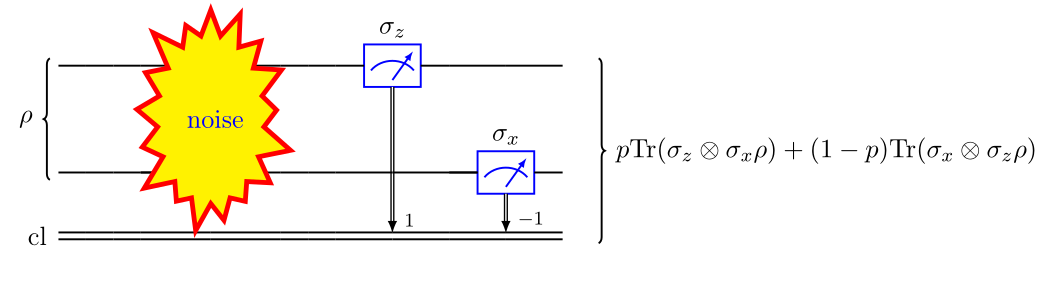
\includegraphics[width=100mm]{images/fm1.png}}
\subfigure[]{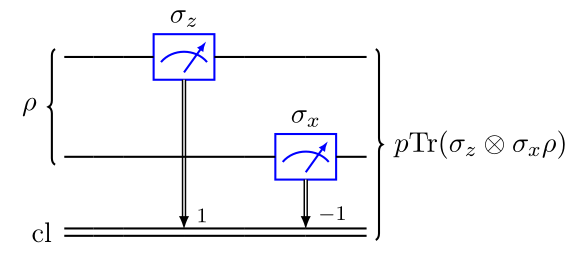
\includegraphics[width=50mm]{images/fmideal.png}}
\subfigure[]{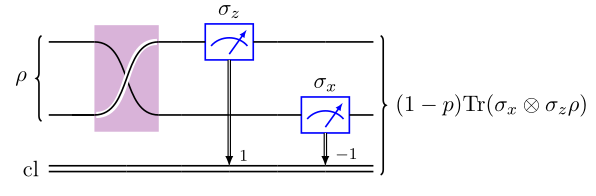
\includegraphics[width=50mm]{images/fm-nonideal.png}}

\caption{Medición difusa}\label{fig:lego}
\end{figure} 

    
\end{frame}

\begin{frame}{Valor esperado y operador difuso}

 
Para un sistema de dos partículas el valor esperado de un observable factorizable es 
\begin{equation*}\label{eq:Expected-Value-FM-2p}
    \begin{split}
      \la {A\otimes B}\ra_{\mathcal{F}_{2\text{p}}(\rho)} =&p\tr(\rho A\tensor B)+(1-p)\tr(\rho B\otimes A).\\
    \end{split}
\end{equation*}Lo que permite introducir al operador difuso que se define como \begin{equation*}\label{eq:op_F2p}
    \mathcal{F}_{2\text{p}}(\rho):=p\rho + (1-p)S_{12}\rho S_{12}^{\dagger}.
\end{equation*}
Para sistemas más grandes es 
\begin{equation*}\label{eq:expected-value-fm-general}
    \la \mathcal{O}\ra_{\fuzzy{\rho}}=\sum_{\Pi_i\in S}p_i\tr(\permut{i}{\rho}\mathcal{O}) =\tr(\fuzzy{\rho}\mathcal{O}).
\end{equation*} donde \begin{equation*}\label{eq:fuzzy-op-nparticles}
    \fuzzy{\rho}=\sum_{\Pi_i\in S}p_{i}\permut{i}{\rho}
 \end{equation*} con $\Pi_i$ son los operadores de permutación.

\end{frame}

\begin{frame}{Instrumentos cuánticos}
  Son un ensamble que correlaciona un sistema clásico y que contiene la salida de la medición y un sistema cuántico que contiene el estado posterior a la medición \begin{equation*}
    \begin{split}
        \mathcal{I}: \mathcal{B(H)}\rightarrow\mathcal{B(H)}_{\text{cl}}\otimes \mathcal{B(H)}_{\text{qu}},\\
    \mathcal{I}(\rho)=\sum_\alpha |\alpha\rala\alpha|\otimes \E_\alpha(\rho).
    \end{split}
\end{equation*}
\end{frame}


\section{Resultados}
\begin{frame}{POVM y operadores de Kraus para mediciones difusas en sistemas de dos partículas}
  Los efectos para una medición difusa son \[\{\mathcal{F}_{2\text{p}}(P_{a_j,b_k}\rho)\}\]los cuales proporciona el mapeo de probabilidades tal que \[   E(a_j b_k, \rho)= \tr(\mathcal{F}_{2\text{p}}({P_{a_j,b_k}})\rho).\] Es necesario descomponer estos efectos, definiendo un conjunto de operadores de Kraus de manera que se cumpla que \[\mathcal{F}_{2\text{p}}(P_{a_j,b_k}\rho)=K_{a_j,b_k}^\dagger K_{a_j,b_k}.\] Por tanto se pueden considerar los siguientes operadores \[K_{a_j,b_k}=\sqrt{\mathcal{F}_{2\text{p}}(P_{a_j,b_k}\rho)}.\]
\end{frame}

\begin{frame}{Instrumentos cuánticos para dos partículas I}

\begin{figure}[H]
\centering
\subfigure[]{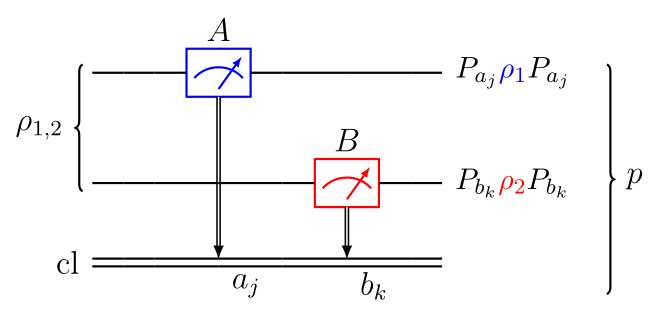
\includegraphics[width=40mm]{images/fmideaqi.png}}
\subfigure[]{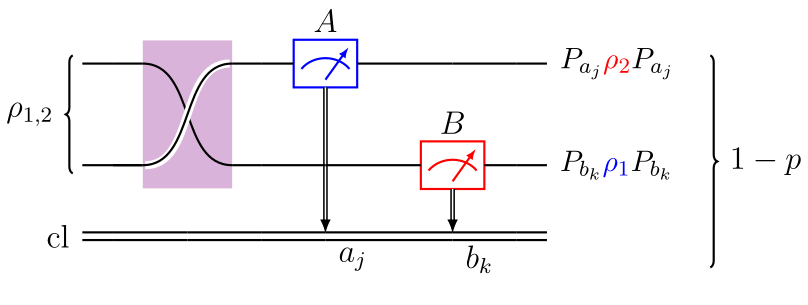
\includegraphics[width=50mm]{images/fmqi1.png}}
\caption*{}
\end{figure} 




\end{frame}

\begin{frame}{Instrumentos cuánticos para dos partículas II}
\begin{figure}[H]
\centering
\subfigure[]{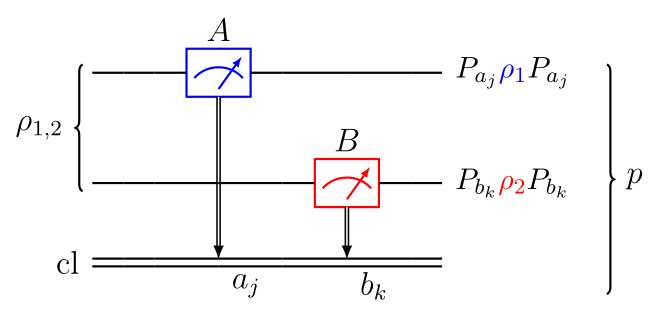
\includegraphics[width=50mm]{images/fmideaqi.png}}
\subfigure[]{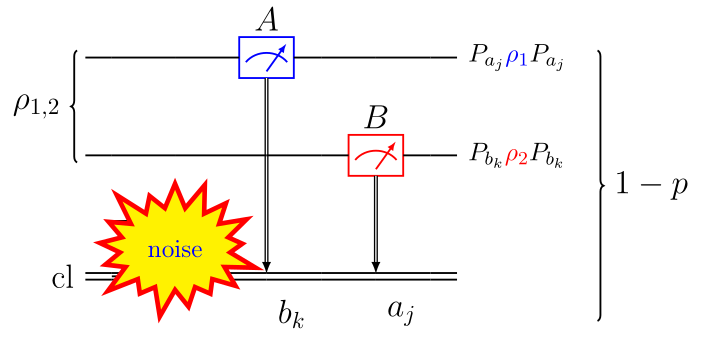
\includegraphics[width=50mm]{images/fmqi2.png}}
\caption*{} 
\end{figure} 

\end{frame}

\begin{frame}{Instrumentos cuánticos para dos partículas III}
\begin{figure}[H]
    \centering
\subfigure[]{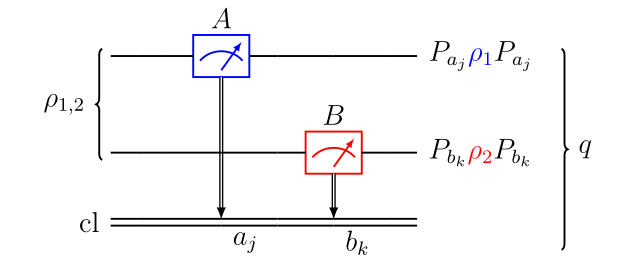
\includegraphics[width=35mm]{images/fmidealiq3.png}}
\subfigure[]{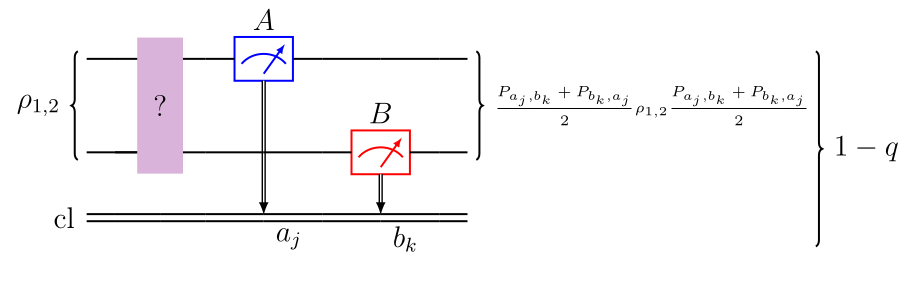
\includegraphics[width=50mm]{images/fmqi3.png}}
\caption*{} 
\end{figure} 
\end{frame}

\begin{frame}{Equivalencia}
    
\end{frame}


\begin{frame}{Generalización}
    
\end{frame}

\section{Conclusiones}

\begin{frame}{Conclusiones}
    
\end{frame}




\end{document}

%%% Local Variables:
%%% mode: latex
%%% TeX-master: t
%%% End:
